\subsection{Flight Sequence} % (fold)
\label{sub:flight_sequence}
The flight of LAD-4 consists of four phases: \textit{powered ascent} after liftoff using the solid motor, \textit{unpowered ascent} from the end of motor burn to apogee, \textit{descent under drogue chute} to an altitude of 700 feet above ground level, and \textit{descent under main chute} until landing. 
\begin{figure}[H]
	\centering
	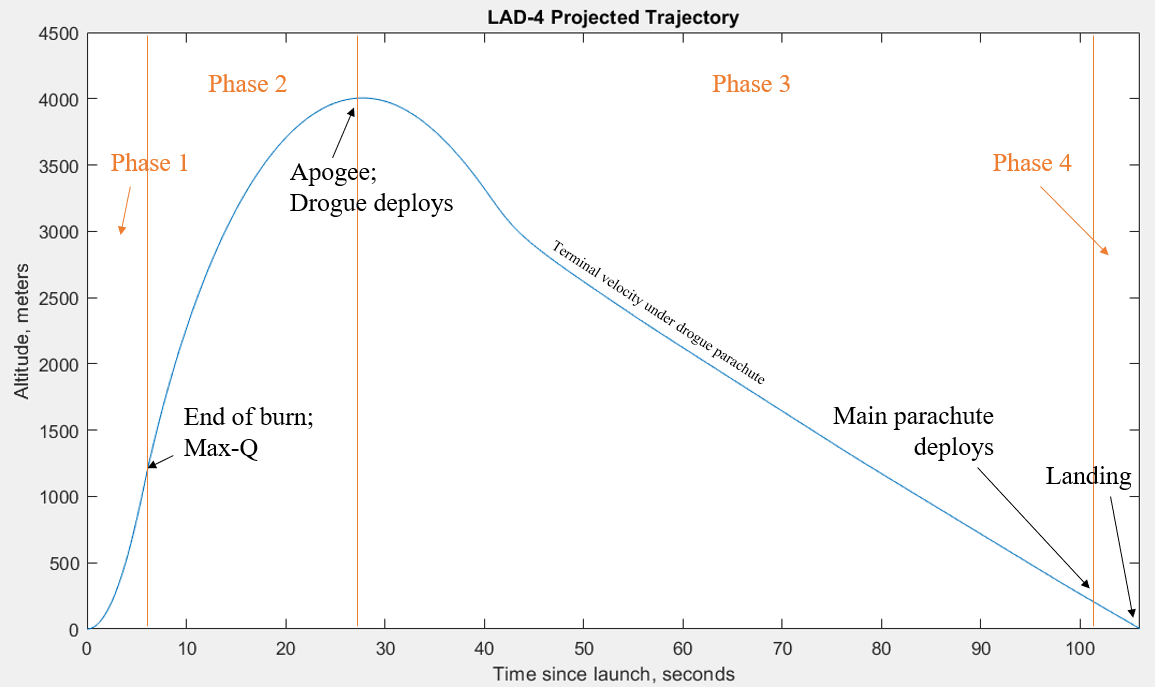
\includegraphics[width=5.5in]{imgs/flightsequence.png}
	\caption{Flight sequence overview with the four phases of flight demarcated.}
	\label{fig:flightsequence}
\end{figure}
\begin{figure}[H]
	\centering
	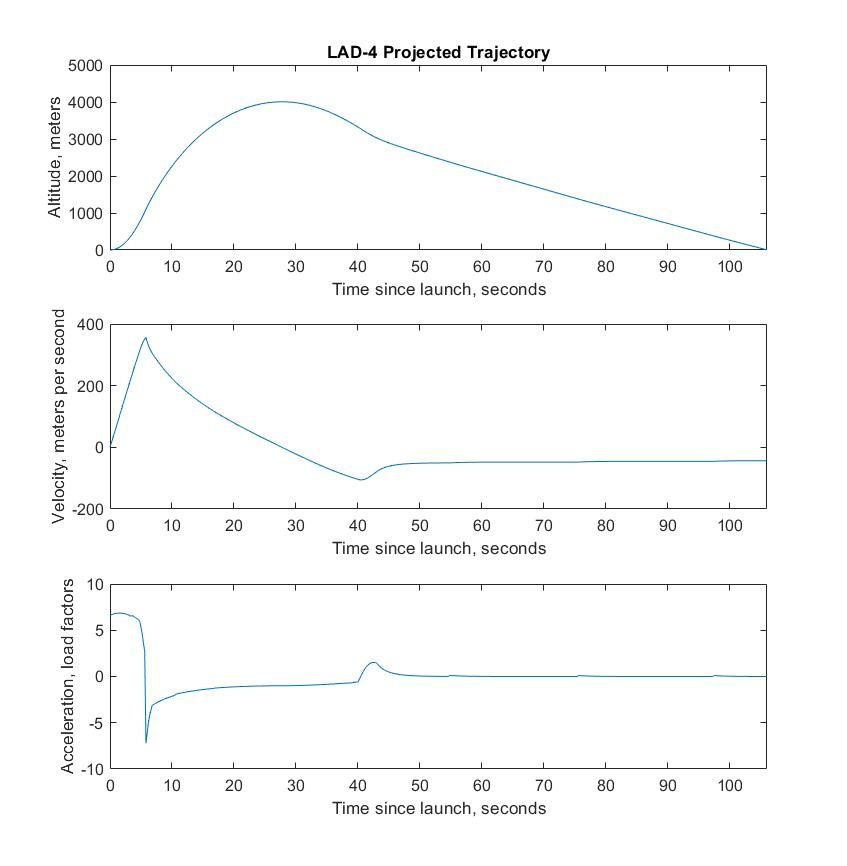
\includegraphics[width=5.5in]{imgs/kinematicsvtime.jpg}
	\caption{Graphs of predicted kinematic parameters as a function of time over the rocket’s flight.}
	\label{fig:kinematics}
\end{figure}
\subsubsection*{Phase 1: Powered Ascent}
When the igniter is powered, combustion of the solid propellant grain commences, and the flight sequence begins. Seconds later, the rocket exits the 20-foot (6.09 m) launch rail with a speed of 27.89 m/s (91.52 ft/s). The Aerotech M1340W-PS motor is designed to burn for 5.7 seconds, with a total impulse of 7673 newton-seconds applied over this time. At the end of the 5.7 second burn, the rocket’s velocity is estimated to be 1161.18 ft/s (353.93 m/s). At this point in the trajectory, the rocket is estimated to be at an altitude of 3491.24 feet above ground level. During this time, the onboard avionics system records altitude data using a barometric altimeter. 
\subsubsection*{Phase 2: Unpowered Ascent (Coasting)}
After the motor finishes its burn, LAD-4 continues on a ballistic trajectory for another 22.1 seconds, which is 28.8 seconds after launch. No longer powered, it loses speed as it approaches its calculated apogee of 13141.66 feet (4005.58 meters) above ground level. Loads on the airframe decrease, and due to the ejection of the propellant mass, the rocket’s center of mass shifts forward. The avionics system continues to record altitude data during this phase of the flight. Apogee is reached, and the unpowered ascent phase of flight ends a few seconds later, when the barometer records an increase in pressure associated with a decrease in altitude over time. At this point, the pyrotechnic charge deploys, shearing the nylon bolts of the forward coupler.
\subsubsection*{Phase 3: Descent Under Drogue Chute}
As a result of the charge deployment and the shearing of the nylon bolts, the nosecone, tethered to the rocket by a shock cord, separates. The drogue parachute deploys and inflates, allowing the rocket to remain in a stable, vertical attitude for the majority of its descent. The rocket reaches its terminal velocity under the small drogue chute about 5 seconds after drogue deployment. During this phase of flight, the avionics system continues to record altitude data.
\subsubsection*{Phase 4: Descent Under Main Chute}
At an altitude of 700 feet above ground level, the avionics system sends a signal to fire the charge in the Tender Descender system. The Tender Descender separates, releasing the main parachute, which inflates outside of the rocket, decreasing its speed for landing. The drogue parachute, attached to the nosecone and to the main airframe by shock cord, deflates, and the entire rocket continues to lose altitude. This phase of flight continues until the rocket lands. The vehicle is then able to be located and recovered.
\subsection{Launch Readiness Procedures} % (fold)
\label{sub:launch_readiness_procedures}
Prior to flight, a document outlining the launch day procedures was constructed. The launch day procedures involved final assembly of the rocket and verification of communication with and arming of the onboard electronic system, written as a checklist of steps necessary to prepare the rocket for launch. The checklist is performed as a call-and-response between at least two \textit{independent} sets of people during launch preparation. 